\documentclass[mathserif, aspectratio=169]{beamer}

\usepackage{psfrag,graphicx}
\usepackage{amsmath}
\usepackage[absolute,overlay]{textpos}

\usepackage{braket}
\graphicspath{{figs/}}

\usetheme{Boadilla}
\makeatother
\setbeamertemplate{footline}[frame number]

\usepackage{graphicx}
\usepackage{caption}
\usepackage{subcaption}
\captionsetup{compatibility=false}
\usepackage{amsmath} 
\usepackage{amssymb} 
\usepackage{amsthm}  
\usepackage{bm}
\usepackage{lipsum}
\usepackage[linesnumbered, ruled]{algorithm2e}
\usepackage{color}
\newtheorem{assumption}{Assumptions}
\newtheorem{prop}{Proposition}
\newtheorem{defn}{Definition}
\newtheorem{thm}{Theorem}
\newtheorem{lem}{Lemma}
\newtheorem{cor}{Corollary}
\newtheorem{sol}{Decentralized Solution}
\newtheorem{thresh}{$\epsilon$-thresholding}
\definecolor{light-gray}{gray}{0.8}
\usepackage{textcomp}

\newcommand{\backupbegin}{
   \newcounter{finalframe}
   \setcounter{finalframe}{\value{framenumber}}
}
\newcommand{\backupend}{
   \setcounter{framenumber}{\value{finalframe}}
}
\newcommand{\norm}[1]{\left\lVert #1 \right\rVert}

\makeatletter
\setbeamertemplate{navigation symbols}{}

\title[Lecture 23] % (optional, use only with long paper titles)
{Data, Environment and Society: \\{Lecture 27: Support Vector Machines, continued}}



\author[ER190C: Data, Environment and Society] 
{Instructor: Duncan Callaway\\
GSI: Seigi Karasaki} 

%\logo{
%\includegraphics[width=1.5cm,height=1.5cm,keepaspectratio]{uvic_logo_h.jpg}
%}
\vspace{-20mm}
\institute[UC Berkeley] % (optional, but mostly needed)
 {\small{ \bf November 27, 2018}}

\date[November 27, 2018]

\begin{document}

\frame{
	\titlepage
}

\begin{frame}{Announcements}
	\begin{itemize}
		\item HW10 due today.
		\item HW11: Optional, for extra credit.  
		\item Seigi and I will be at lab next week
		\begin{itemize}
			\item Attendance optional -- but we will help with projects.
		\end{itemize}
		\item Final lecture, here on Tuesday 12/4.  
		\begin{itemize}
			\item Covers neural nets and course wrap-up
			\item But I'll also post a video 
			\item No reading for this.
		\end{itemize}
		\item Projects: Due December 11 at 6pm.
	\end{itemize}
\end{frame}

\begin{frame}{	A few more project notes:}
	\begin{itemize}
		\item Don't forget to normalize your data if you're using lasso, ridge, elastic net. 
		\item It's important to get your resource allocation right, but more important to run some models.
		\item That is, don't let the perfect be the enemy of the good!
		\item We'll be in Barrows 110 next monday 10-12 for consultations on your projects.
	\end{itemize}	
\end{frame}

\begin{frame}{Objectives for today}
	\begin{enumerate}
		\item Review fundamentals building up to SVM (from two weeks ago!)
		      \begin{itemize}
			      \item Hyperplanes
			      \item Maximal margin hyperplanes for linearly separable data
			      \item Support vector classifiers: linear boundaries for non-separable data
		      \end{itemize}
		\item Open your horizons to the \textbf{support vector machine}
		      \begin{itemize}
			      \item This provides \textbf{nonlinear} separations of the feature space
		      \end{itemize}
	    \item Discuss the basic pipeline for model building with cross validation
	    \begin{itemize}
	    	\item Train, test and validation data sets
	    	\item Fit the model
	    	\item Choose ``hyperparameters''
	    	\item valuate error distributions
    	\end{itemize}
    	\item Course reviews
	\end{enumerate}

\end{frame}


\begin{frame}{Theoretical example: Classification with hyperplanes}
	\begin{columns}
		\column{0.5\textwidth}
		Suppose we have
		\begin{itemize}
			\item \textcolor{blue}{blue points}
			\item \textcolor{red}{red points}
		\end{itemize}
		\vspace{10mm}
		A ``separating hyperplane'' has the property that:

		\column{0.5\textwidth}

	\end{columns}

\end{frame}


\begin{frame}{Using the plane for predictions}
	\begin{columns}
		\column{0.5\textwidth}
		This part is simple.  If we have a test observation, we simply evaluate $f(x_\text{test})$ and assign it to a class on the basis of the sign of the result.
		\column{0.5\textwidth}

	\end{columns}
\end{frame}


\begin{frame}{Maximal margin hyperplane (MMH)}

	\begin{columns}
		\column{0.5\textwidth}
		\begin{itemize}
			\item MMH defined: The MMH is the hyperplane that \textit{maximizes} the distance to the closest point.
			      \begin{itemize}
				      \item In other words: it is the plane that is farthest from the data.
			      \end{itemize}
			\item Important: This requires that the data are \textit{linearly separable.  }
			\item 2-3 points defining the hyperplane are termed ``support vectors'' because each observation is a ``vector'' of information that supports the plane.
		\end{itemize}
		\column{0.5\textwidth}

	\end{columns}
\end{frame}



\begin{frame}{Support vector classifier details}

	\begin{columns}
		\column{0.5\textwidth}
		We'll solve a slightly different optimization problem.
		\begin{itemize}
			\item Still classifies observations on the basis of what side of the hyperplane they're on
			\item But a few observations can be mis-classified.
			\item But with $C$, the $\epsilon$ values are chosen within a budget.
			      \begin{itemize}
				      \item $\epsilon_i = 0$, no margin violation
				      \item $0<\epsilon_i<1$, in the margin but on the correct side of the plane
				      \item  $\epsilon_i>1$, on the wrong side of the plane.
			      \end{itemize}
		\end{itemize}
		\column{0.5\textwidth}
		The optimization problem is:
		\vspace{40mm}
	\end{columns}
\end{frame}


\begin{frame}{Setup for SVM ``Kernels'': Linear boundary}

	\begin{columns}
		\column{0.5\textwidth}
		\vspace{10mm}

		Let $\braket{x_i,x_k} = \sum_{j=1}^px_{ij}x_{kj}$

		\vspace{5mm}

		One can show that:

		\begin{align*}
			\beta_0 + \sum_{j=1}^p \beta_j x_{ij} & \Leftrightarrow \beta_0 + \sum_{k=1}^n \alpha_k \braket{x_i,x_k} \\
			f(x_i)                                & = \beta_0 + \sum_{k\in \mathbb{S}} \alpha_k \braket{x_i,x_k}     \\
		\end{align*}

		\column{0.5\textwidth}
		What's the relationship between $\alpha$ and $\beta$?
		\vspace{50mm}
	\end{columns}
\end{frame}


\begin{frame}{Decision boundaries aren't always so simple...}

	\begin{columns}
		\column{0.5\textwidth}
		What if the boundary looked like this?
		\vspace{40mm}
		\column{0.5\textwidth}
		We might get better performance if we replaced the linear plane in the optimization problem with something else.

	\end{columns}
\end{frame}


\begin{frame}{SVM Kernels}
	\begin{columns}
		\column{0.7\textwidth}

		\begin{align*}
			K_\text{linear}(x_i,x_k)     & = \braket{x_i,x_k} = \sum_{j=1}^px_{ij}x_{kj} \\
			K_\text{polynomial}(x_i,x_k) & = (1+ \sum_{j=1}^px_{ij}x_{kj})^d             \\
			K_\text{radial}(x_i,x_k)     & = \exp(-\gamma \sum_{j=1}^p(x_{ij}-x_{kj})^2) \\
		\end{align*}

		Then we can apply these kernels:
		\begin{align*}
			f(x_i) = \beta_0+\sum_{k=1}^p \alpha_k K(x_i,x_k)
		\end{align*}
		\column{0.3\textwidth}

		The radial kernel serves to give training observations far from a test point less weight (due to negative exponential).

		\vspace{5mm}

		For the radial kernel, all the data comprise the model -- analogous to KNN.
	\end{columns}

\end{frame}


\begin{frame}{Polynomial kernel expanded}
	\begin{align*}
		K_\text{polynomial}(x_i,x_k) & = (1+ \sum_{j=1}^px_{ij}x_{kj})^d \\\\
		d = 1 \Rightarrow K_\text{polynomial}(x_i,x_k) &= \\\\
		d = 3 \Rightarrow K_\text{polynomial}(x_i,x_k) &= 
	\end{align*}

\vspace*{10mm}
	...So adjusting $d$ is essentially ``feature engineering'' to manipulate what order terms you put in your classifier.	
\end{frame}

\begin{frame}{Radial Basis Functions}
	\begin{align*}
		K_\text{radial}(x_i,x_k) & = \exp(-\gamma \sum_{j=1}^p(x_{ij}-x_{kj})^2),\\ f_\text{radial}(x_i) &= \beta_0+\sum_{k=1}^p \alpha_k K_\text{radial}(x_i,x_k)
	\end{align*}

	Observations $k$ in the training set that are close to observation $i$ will get...
	\begin{itemize}
		\item More weight?
		\item Less weight?
	\end{itemize}	

	Assume $\alpha$ is positive.  Then points closer to $x_i$ will yield
	\begin{itemize}
		\item larger $f$?
		\item smaller $f$?
	\end{itemize}
Larger evaluations of the kernel push $f$ in the positive direction $\rightarrow$ tend to classify with the positive variable.
\end{frame}

\begin{frame}{What do the kernels look like?}
	\begin{columns}
		\column{0.7\textwidth}

		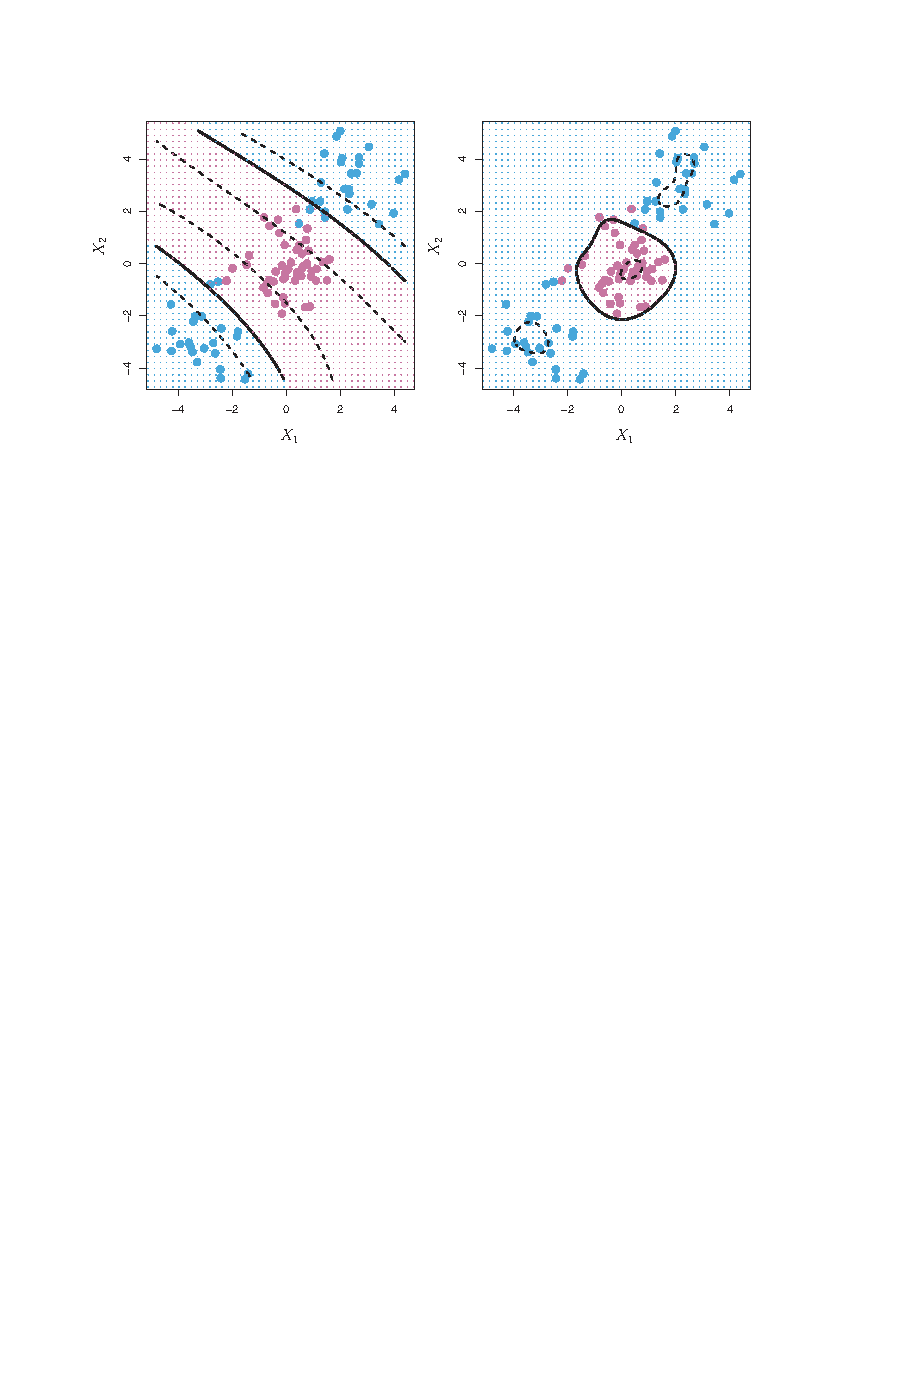
\includegraphics[scale=0.8]{SVM_kernels}

		\column{0.3\textwidth}

		Left: Polynomial, $d=3$.  Right: Radial.

		\vspace{5mm}
		Note that $d$ and $\gamma$ are parameters to tune (via cross validation!)
	\end{columns}
\end{frame}

\begin{frame}{SVM Example}

	\begin{figure}
		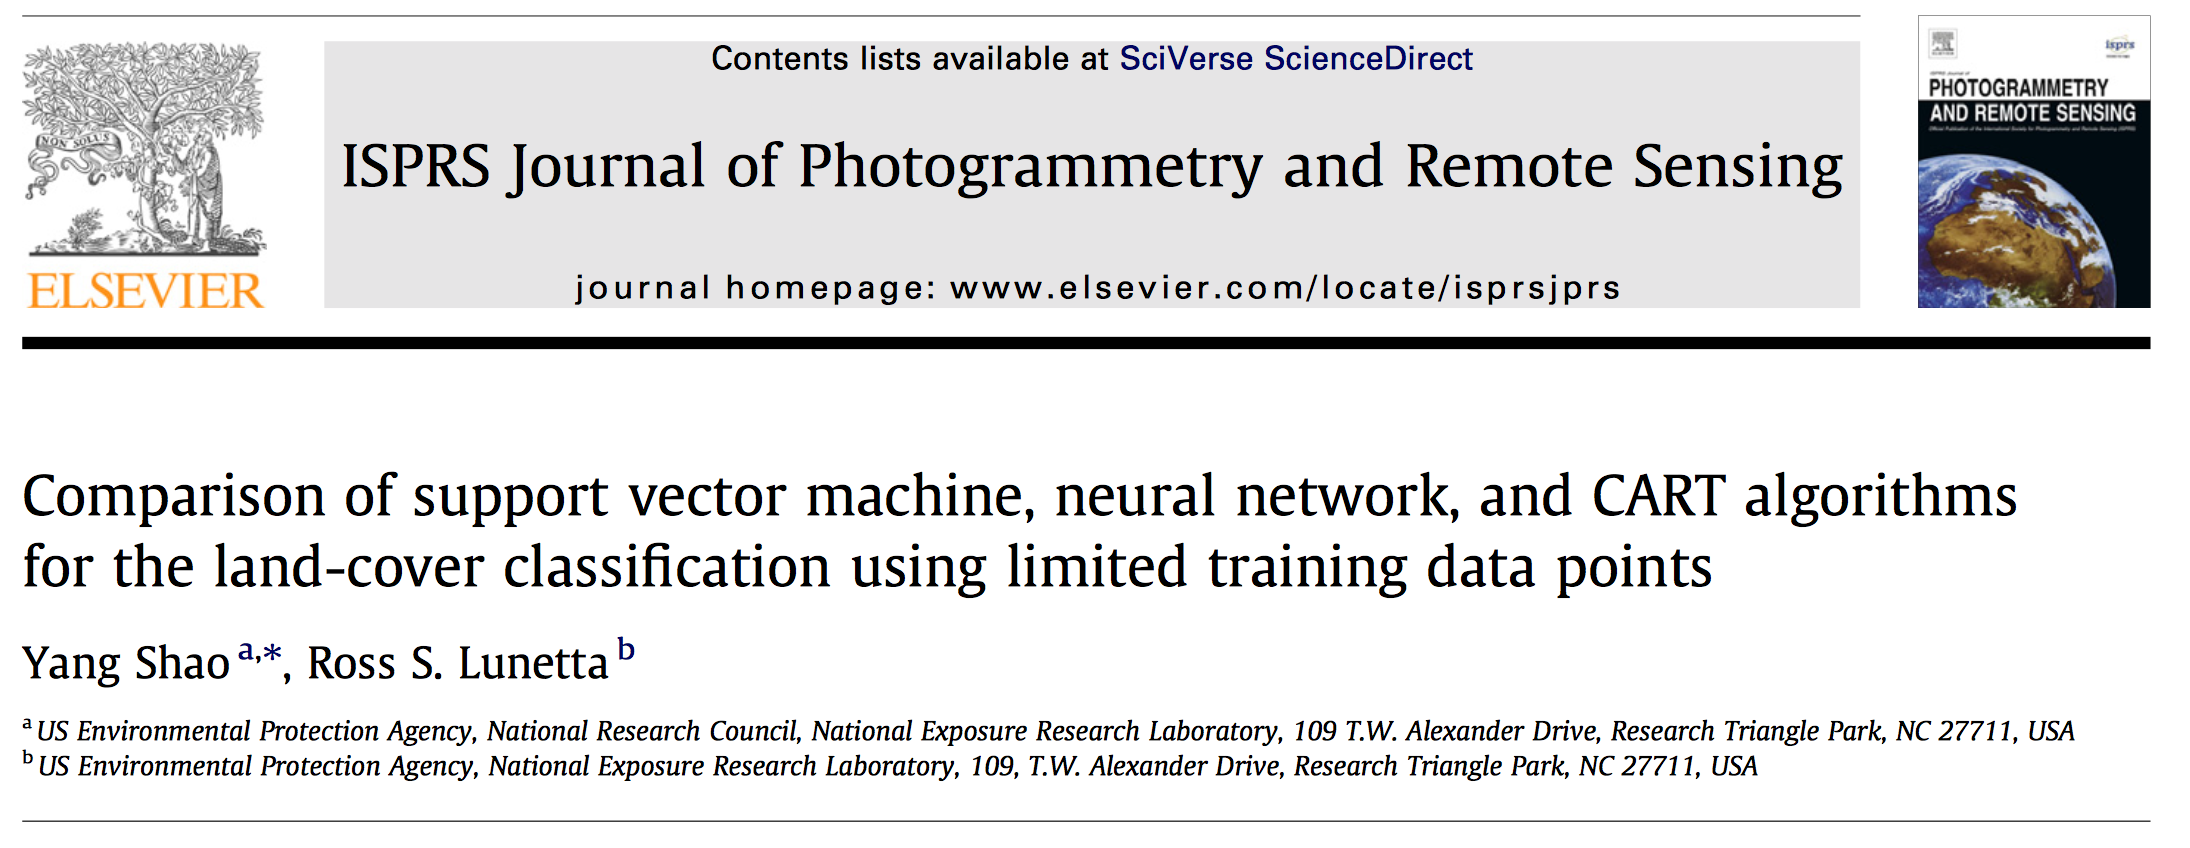
\includegraphics[width=\textwidth]{shao_JPRS}
		\caption*{}
	\end{figure}
\end{frame}


\begin{frame}{Shao and Lunetta setup}
	Loads of remote sensing data (MODIS):
	\begin{itemize}
		\item 46 input features for each 250 m$^2$ pixel
		      \begin{itemize}
			      \item 23 short wave infrared (SWIR) surface reflectance
			      \item 23 Enhanced Vegetation Index metrics -- basically a summary of the wavelengths
		      \end{itemize}
		\item Training data from National Land Cover Dataset (NLCD), classifying land as
		      \begin{itemize}
			      \item urban,
			      \item deciduous forest,
			      \item evergreen forest,
			      \item agricultural land, and
			      \item wetland
		      \end{itemize}

		\item Question: How do SVM, Neural networks (coming soon!), and regression trees perform relative to one another?
	\end{itemize}
\end{frame}


\begin{frame}{Shao and Lunetta SVM Result}

	\begin{figure}
		\includegraphics[height=0.9\textheight]{shao_figure}
		\caption*{}
	\end{figure}
\end{frame}

\begin{frame}{}
	\begin{figure}
		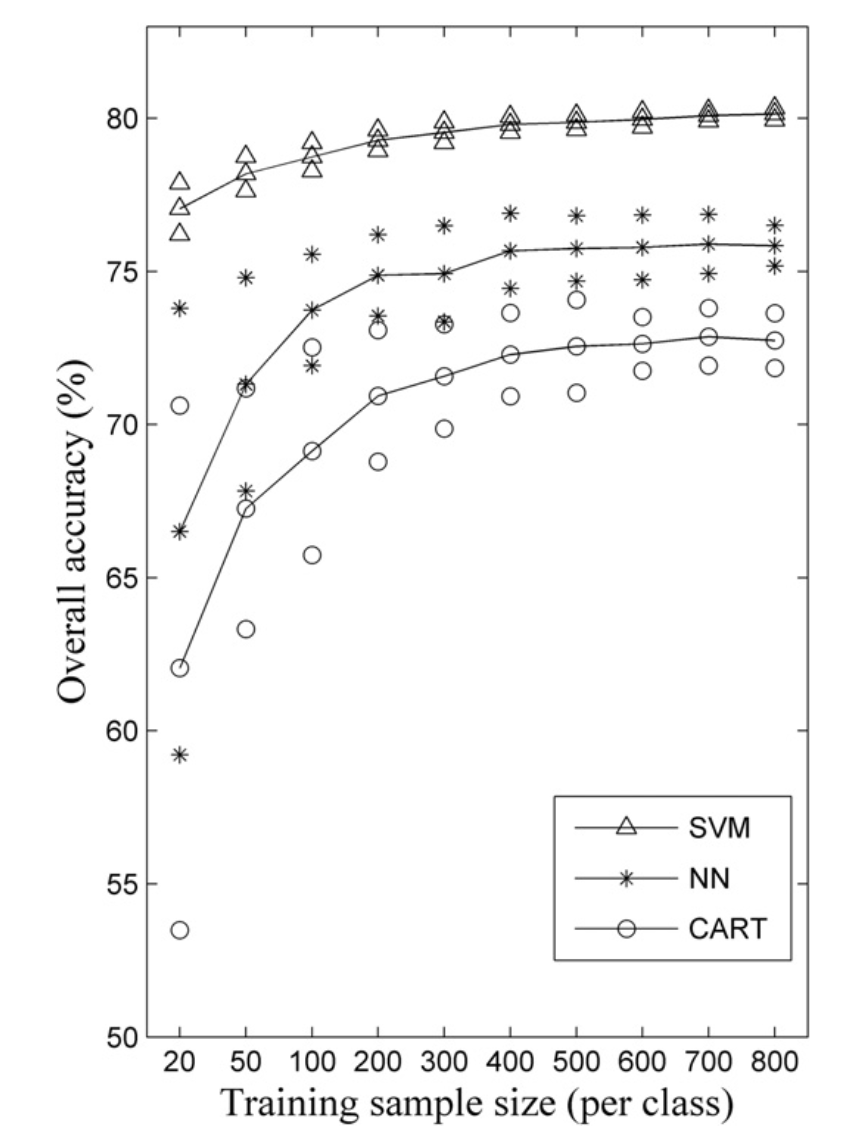
\includegraphics[height=\textheight]{shao_performance}
		\caption*{}
	\end{figure}
\end{frame}

\begin{frame}{Textbook example: Heart Data}
	First: Receiver operating characteristic (ROC)\\~\\

	\textbf{Sensitivity} = the fraction of ``positives'' that are correctly identified as positives  \\~\\

	\textbf{Specificity} = fraction of negatives that we correctly identify as negatives \\~\\

	\textbf{True positive rate} = sensitivity\\~\\

	\textbf{False positive rate} = $1-$ specificity

	Ideal classifiers have large true positive rate and low false positive.  \\~\\

	For a given method, there are usually parameters one can tune to explore the tradeoff between true and false positives.
\end{frame}

\begin{frame}{Classifying heart disease}
	\begin{figure}
		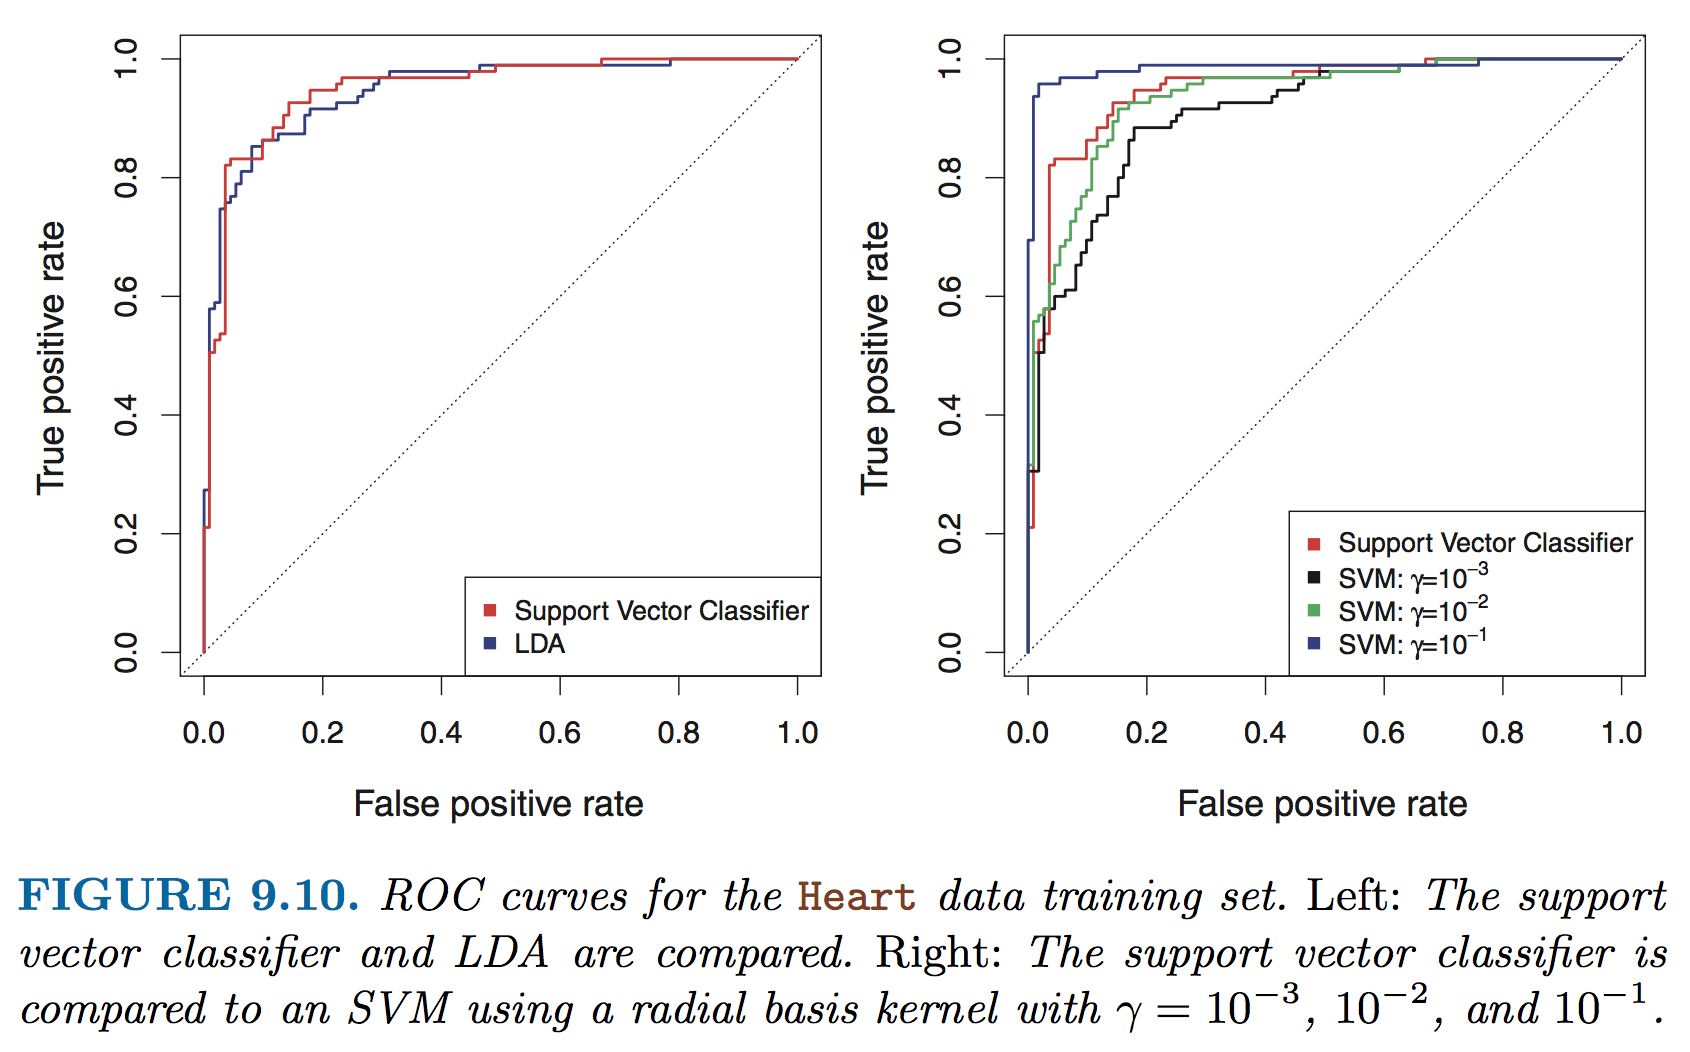
\includegraphics[width=0.7\textwidth]{fig9_10}
		\caption*{}
	\end{figure}
\end{frame}

\begin{frame}{Classifying heart disease -- test data}
	\begin{figure}
		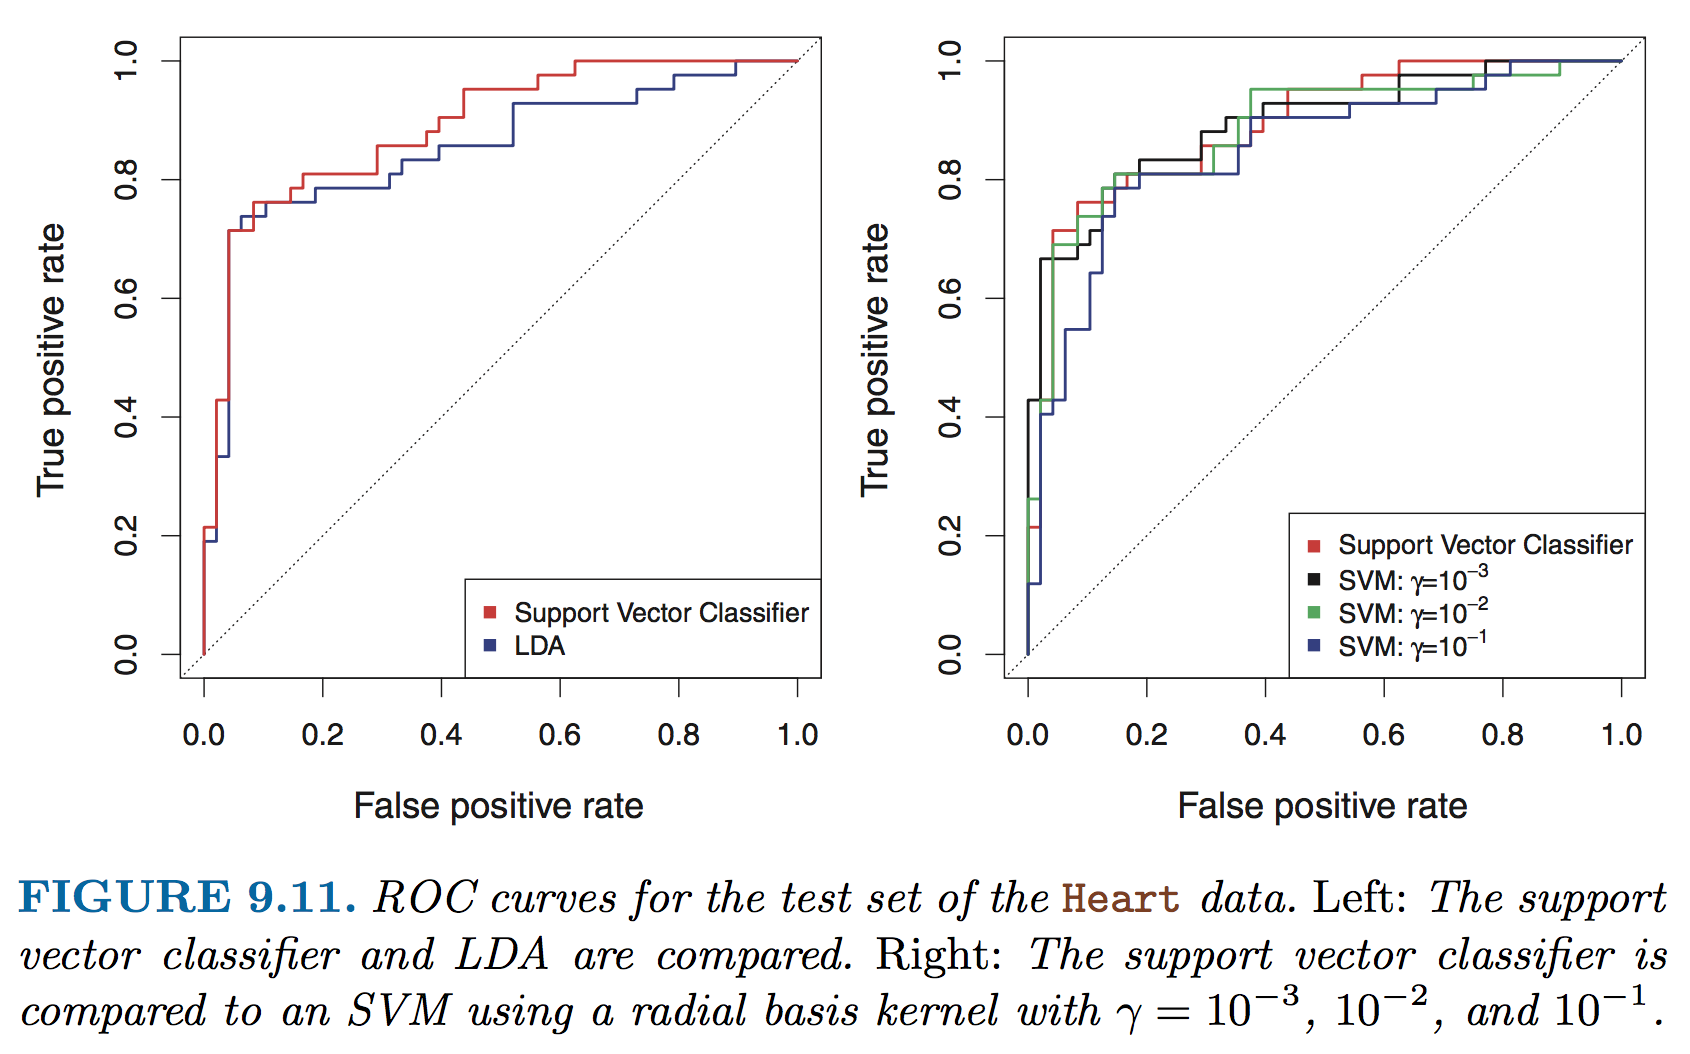
\includegraphics[width=0.7\textwidth]{fig9_11}
		\caption*{}
	\end{figure}
\end{frame}

\begin{frame}{Interpreting Heart data result}

	On training data, SVM with radial kernels are exceptional \\~\\

	...But not so much on test data.  Why?\\~\\
	\pause

	The decision boundary is really ``wiggly'' and prone to overfit. \\~\\

	It appears that SVC would have lower variance / higher bias and they balance perfectly in  this particular case.

\end{frame}

\begin{frame}{Speaking of wiggly boundaries: From Elements of Statistical Learning}

	\begin{figure}
		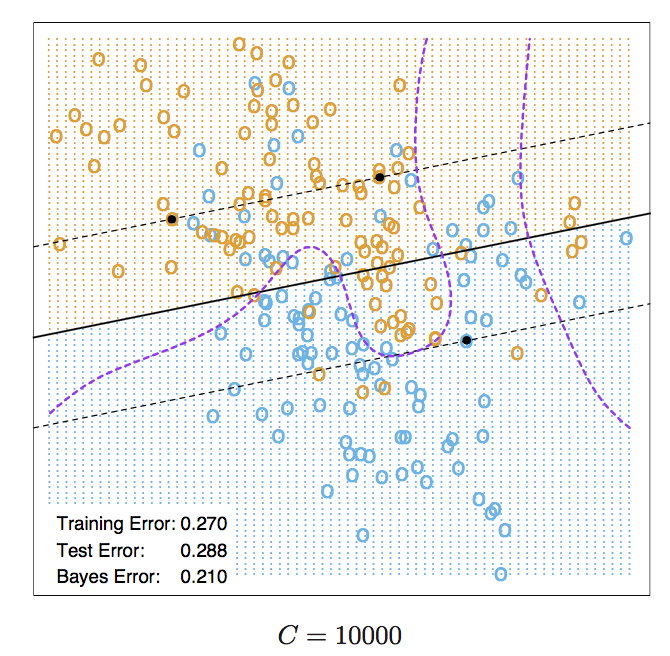
\includegraphics[width=0.415\textwidth]{ESL_12_2a}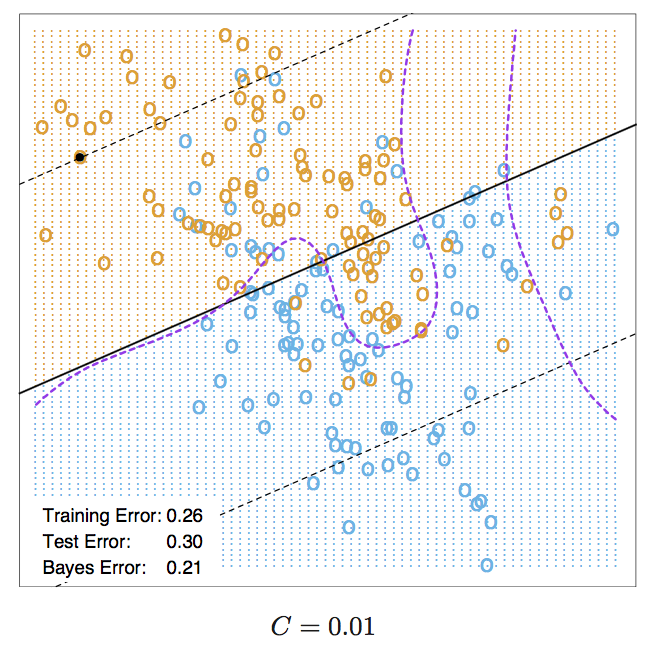
\includegraphics[width=0.4\textwidth]{ESL_12_2b}
		\caption*{These boundaries constructed with SVC.  Purple is ``truth'' (what they used to generate the data).  Note!  In ESL $C$ is the inverse of $C$ in ISLR.  So large $C$ here corresponds to small $C$ there, and vice versa.}
	\end{figure}

\end{frame}

\begin{frame}{One more example: From Elements of Statistical Learning}

	\begin{figure}
		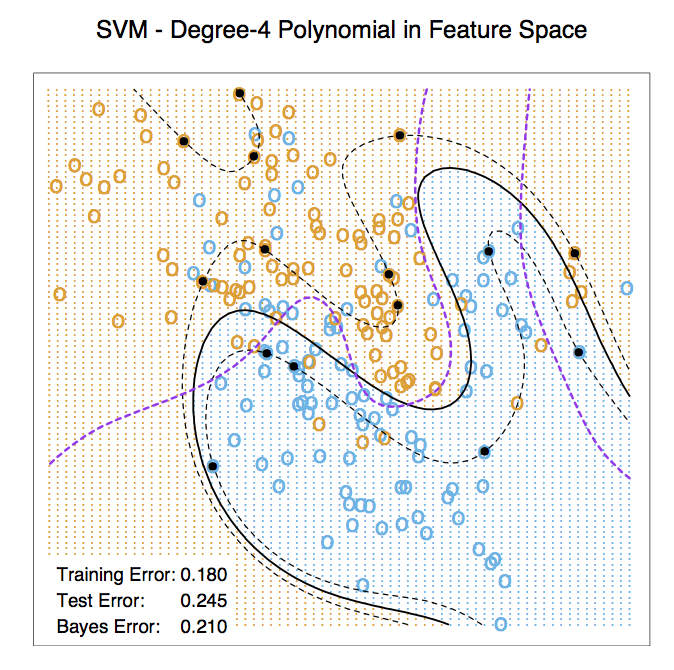
\includegraphics[width=0.4075\textwidth]{ESL_12_3a}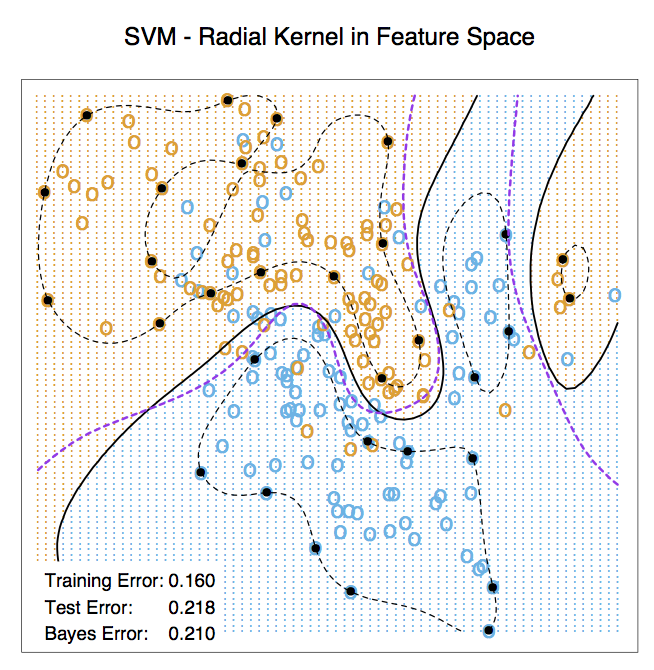
\includegraphics[width=0.4\textwidth]{ESL_12_3b}
		\caption*{These boundaries constructed with SVM. Purple is ``truth'' (what they used to generate the data).  }
	\end{figure}

\end{frame}

\begin{frame}{Models have two different classes of parameters}
	\begin{enumerate}
		\item Parameters that enter as decision variables for minimizing loss function:
		\begin{align*}
			\text{Shrinkage: } & \beta^*  &=& \arg \min_\beta \sum_{i=1}^N \left(Y_i - X_i \beta \right)^2+\lambda \cdot R(\beta)\\
			\text{CART: } & \{j^*,s^*\}  &=& \arg \min_{j\in J, s\in X_j} \sum_{i:x_i\in R_1(j,s)} (y_i-\hat{y}_{R_1})^2 + \sum_{i:x_i\in R_2(j,s)} (y_i-\hat{y}_{R_2})^2
		\end{align*}
		\item ``Hyperparameters'': parameters that constrain how you solve the loss function.  These generally prevent overfit.
		\begin{itemize} \pause
			\item $\lambda$ in shrinkage methods
			\item How deep to grow a classification tree?
			\item $\sum_{i=1}^n \epsilon_i$ in SVM
		\end{itemize}
	\end{enumerate}
	
\end{frame}

\begin{frame}{Ways to minimize the loss function}
	\begin{columns}
		\column{0.5\textwidth}
			\begin{itemize}
				\item Closed form solution -- e.g. normal equations
				\item Gradient search
			\end{itemize}

		\column{0.5\textwidth}
	\end{columns}

	In both cases, we're relying on the condition that the gradient of the loss function approaches zero as we approach the optimal solution 
\end{frame}


\begin{frame}{Ways to choose hyperparameters}
	\begin{columns}
		\column{0.5\textwidth}
			\begin{itemize}
				\item \textbf{Grid search}: This is what we've done with shrinkage methods, when there is just one parameter to tune ($\lambda$)
				\item \textbf{Randomized parameter search}: This is what you're doing in HW10.  Works well when you have lots of hyperparameters to tune.
			\end{itemize}
		\column{0.5\textwidth}
			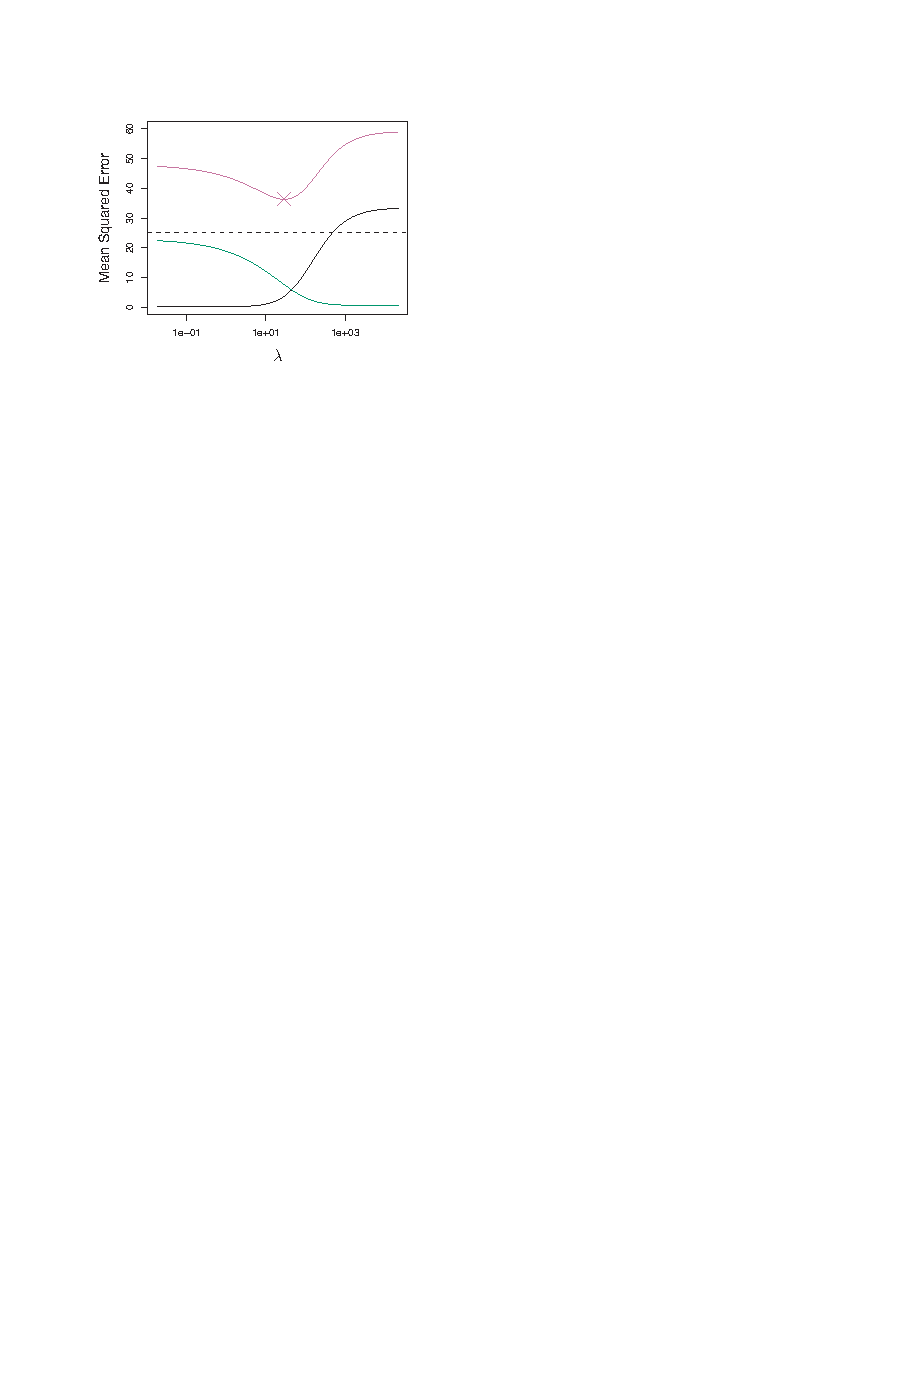
\includegraphics[width=0.9\textwidth]{bias-variance-ridge}
	\end{columns}
	In both cases, all we're doing is 
	\begin{itemize}
		\item Creating a list of candidate hyperparameters (or sets of hyperparameters)
		\item Training the model (with the training data) for each hyperparameter in the list
		\item Choosing the hyperparameter with the best cross-validated error.
	\end{itemize}
\end{frame}

\begin{frame}{Zoom out: Train, (cross) validate and test}
	Using slightly different language, some definitions from from Brian Ripley, Pattern Recognition and Neural Networks, 1996, page 354:
	\vspace{5mm}
	\begin{itemize} 
		\item \textbf{Training set}: ``A set of examples used for learning, that is to fit the parameters of the classifier.''
		\begin{itemize}
			\item<2->{For minimizing the loss function}
		\end{itemize}
		\item\textbf{ Validation set}: ``A set of examples used to tune the parameters of a classifier, for example to choose the number of hidden units in a neural network.''
		\begin{itemize}
			\item<3-> For choosing hyperparameters.
		\end{itemize}
		\item \textbf{Test set}: ``A set of examples used only to assess the performance of a fully-specified classifier.''
		\begin{itemize}
			\item<4->For a final check -- no more model fitting allowed here!
		\end{itemize}
	\end{itemize}
	\vspace{5mm}
	I'll use these definitions going forward.  
\end{frame}

\begin{frame}{Why use validation \textit{and} test sets?}

I.e., why isn't it enough to use just a validation set? \pause
	\begin{itemize}
		\item Because we iteratively tune hyperparameters with the validation sets, the models ``see'' the data
		\item So in essence the validation sets \textit{are} training the model
		\item Keeping a test set locked away until the end of the model fitting process is the only way to be sure the comparison of your models is fair.
		\item We haven't done this in the course -- but if you wish to compare different types of models (e.g. SVM vs random forest) then it's good practice.
	\end{itemize}
\end{frame}

\end{document}
